\chapter{Arquitetura e decisões de projeto}
\label{cap:arquitetura}
\rubricaJustificativa
\section{Arquitetura física e lógica}
A Figura~\ref{fig:arquitetura} explicita os dois fluxos: (i) captação local contínua DHT11~$\rightarrow$~ESP32~$\rightarrow$~OLED; (ii) telemetria ao EMQX via Wi-Fi, consumida pelo MQTTX e pelo \texttt{gravador.py}. Com a rede interrompida, a tarefa do sensor permanece independente da tarefa de rede; mensagens pendentes podem ser enfileiradas localmente.
\begin{figure}[H]\centering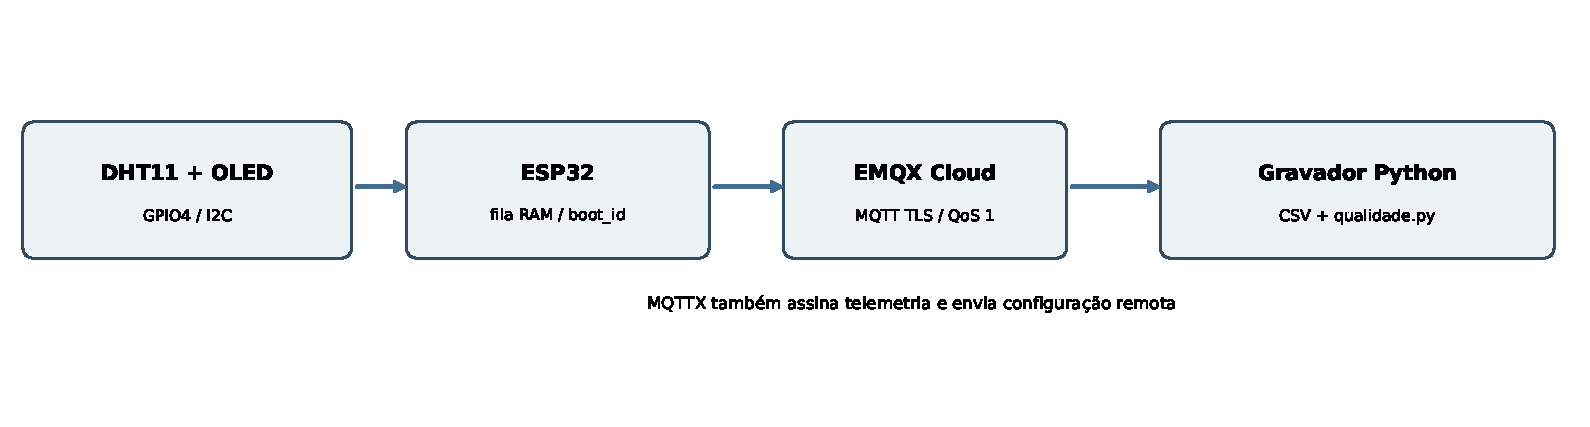
\includegraphics[width=0.94\textwidth]{figuras/arquitetura.pdf}\caption{Arquitetura lógica efetivamente implementada no ciclo 2.}\label{fig:arquitetura}\fonte{Elaborada pela equipe.}\end{figure}
\section{Hardware e barramentos}
O DHT11 utiliza a GPIO4; o OLED SSD1306 de 128$\times$64 usa I\textsuperscript{2}C em SDA/GPIO21 e SCL/GPIO22, endereço \texttt{0x3C}. Ambos usam 3,3~V e terra comum. A leitura do sensor é agendada a cada 2~s; a apresentação visual só é redesenhada quando a indicação muda. As conexões físicas estão consolidadas no Apêndice~\ref{ap:barramento}.
\section{Decisões estruturais}
\begin{decisao}{Separação entre sensoriamento e rede}
\alternativas{Laço de leitura bloqueado por conexão; tarefas cooperativas por \texttt{millis()}.}
\criterio{Continuar lendo o DHT11 a cada 2~s mesmo durante 2~min sem Wi-Fi.}
\escolha{Execução local e reconexão periódica sem laço bloqueante de espera.}
\evidencia{O firmware mantém tarefa de sensor, OLED, Wi-Fi, MQTT e fila separadas.}
\consequencia{A fila de 120 registros limita recuperação; sem alimentação as leituras não publicadas são perdidas.}
\end{decisao}
\begin{decisao}{Identificador por inicialização}
\alternativas{Somente \texttt{seq}; sequência persistente por escrita frequente; \texttt{boot\_id} persistente e \texttt{seq} volátil.}
\criterio{Separar dois registros \texttt{seq=1} em reinícios distintos sem gravar NVS a cada 30~s.}
\escolha{Persistir \texttt{boot\_id} uma vez por inicialização, via \texttt{Preferences}.}
\evidencia{Arquivo final registra \texttt{boot\_id}=120, 121 e 122 e duas duplicatas reais pela chave composta.}
\consequencia{Zerar fisicamente a NVS ou desgaste/falha de gravação pode quebrar a monotonicidade; não representa UUID global.}
\end{decisao}
\begin{decisao}{Persistência no assinante}
\alternativas{Exclusivamente visualizar no MQTTX; CSV por assinante com sessão persistente.}
\criterio{Sustentar uma coleta que atravessa períodos com notebook desconectado, sem descartar eventos e metadados.}
\escolha{Assinante Python com cliente fixo, QoS~1, \texttt{manual\_ack=True}, \texttt{flush()} e \texttt{fsync()} por registro.}
\evidencia{O CSV final contém 3.096 mensagens; o log documenta retorno com backlog após pausa do gravador.}
\consequencia{A latência de gravação e as políticas de retenção do broker são fatores externos; duplicatas continuam possíveis com QoS~1.}
\end{decisao}
